\chapter{Subscriptor Podcast}

\section{TIC}

Tecnologías de la Información y Comunicación (TIC): radio, televisión e
Internet. Satisfacen una de las necesidades de la sociedad.

\subsection{TIC en la Educación}

Las TIC ayudan a diversificar la enseñanza y el aprendizaje de lenguas 
originarias y extranjeras, por lo tanto, países de América Latina y el
Caribe optan por implementar políticas gubernamentales de equipamiento a
instituciones educativas.

Según \cite{severin2013enfoques} muchos países hicieron esfuerzos por
incorporar las TIC a procesos de enseñanza y aprendizaje. 

\section{Web 2.0}

La Web 2.0 denominada sistema de principios y practicas brinda comunicación y
servicios sobre la red de Internet: Facebook, Flicker, Youtube, Blogger, Twitter.

\subsection{La creación de contenidos digitales}

El trabajo de profesionales de diferentes áreas es considerado como
multidisciplinario; para tal motivo es aconsejable el uso de flujos de trabajo
o estándares de trabajo. 

Segun \cite{duart2000aprender} elaborar materiales didácticos en soporte web
se encuentra con la confluencia de al menos cuatro disciplinas. La primera, es
la tecnología, que acostumbra a tomar la forma concreta la informática. La
segunda es el diseño gráfico. La tercera es la pedagogía, y más concreta-mente
la especialización en tecnología educativa. La cuarta es, finalmente, la
disciplina.

\subsection{Podcast}

Podcast es un archivo digital que tiene las siguientes características: un
reproductor (audio/vídeo), disponible desde un sitio web, tiene la opción
para descargar.

El Podcast es un recurso o herramienta novedosa y muy útil por sus
características en el aprendizaje de lenguas. En el ámbito educativo 
el Podcast \textquotedouble{es un herramienta muy flexible para la 
educación por que permite elaborar guiones adaptados a nuestra realidad 
educativa.} \cite{chacon2011podcast}. Es decir, es un recurso que permite hacer
uso de la creatividad en la producción de guiones con diferentes 
temáticas. \cite{AFSTVV2014}
 
Se menciona el término Podcasting como: crear un Podcast y realizar su difusión.

\section{\textquestiondown Que es un feed de noticia?}

La tecnología \footnote{tecnología: Es la aplicación de un conjunto de
conocimientos y habilidades con un claro objetivo: conseguir una solución que
permita al ser humano desde resolver un problema determinado hasta el lograr
satisfacer una necesidad en un ámbito concreto. \cite{technology}} feed
\footnote{feed: Un archivo coherente, legible por la máquina que
permite a los sitios web para compartir su contenido con otras aplicaciones en
una forma estándar.\cite{hammersley2005developing}} de noticia
actualiza al usuario a los últimos contenidos de un sitio web vía correo
electrónico; Este tiene la siguiente estructura propuesta: título, descripción,
programa de aprendizaje.

Según \cite{hammersley2005developing} el uso de RSS \footnote{RSS: Es un
método de noticias descubriendo un otro contenido Web que está disponible
para la alimentación. \cite{zeki2004rss}} y Atom es proporcionar un feed de
sindicación de contenido: un archivo coherente, legible por la máquina que
permite a los sitios web compartir su contenido con otras aplicaciones de
manera estándar.

RSS como formato basado en XML \footnote{XML: Es un metalenguaje para definir
idiomas para el intercambio de información en la Web, los formatos de fuentes
son también a menudo se llama \textquotedouble{dialectos XML} o 
\textquotedouble{XML vocabularios}. \cite{wittenbrink2005rss}} utiliza la
estructura de un subscriptor de noticia.

Según \cite{wittenbrink2005rss} RSS y Atom son documentos XML; tienen la
función de actualizar y compartir información. Estos documentos también son
mencionados: newfeeds or feed. 

\section{Sintaxis: RSS como documento XML}

Según \cite{wittenbrink2005rss} para muchos desarrolla-dores
\textquotedouble{XML} y \textquotedouble{RSS} son sinónimos. Se utiliza ambas
tecnologías para el intercambio de información en la web.

RSS es un tipo de feed compuesto de una estructura simple.

Se identifica un ícono de color naranja tiene en su interior un circulo 
y dos lineas curvas de color blanco; para conocer que la aplicación web 
cuenta con un subscriptor.

\begin{minipage}{1.0\linewidth}
	\centering
	\fbox{
		
\includegraphics[scale=0.8]{rss}
	}
	\captionof{figure}{Ícono representación gráfica de un feed}
	\source{fuente: \cite{iconRss}}
	\label{Ícono representación gráfica de un feed}
\end{minipage}

\subsection{Información básica de un RSS 2.0}

Según \cite{wittenbrink2005rss} un subscriptor tiene un channel
\footnote{channel: En las telecomunicaciones en general un canal es un camino
separado a través del cual las señales pueden fluir. \cite{channel}} (canal)
el cual debe incluir elementos: título, enlace y descripción. Estos elementos
son obligatorios dentro un channel son elementos necesarios con el fin de
caracterizar la recogida de información.

Según \cite{wittenbrink2005rss} el título del mensaje es individual
corresponde con el subtitulo en un archivo de tipo HTML \footnote{HTML: Es el
conjunto de símbolos de marcado o códigos insertados en un archivo destinado
a la visualización de una página Web Mundial. \cite{html}}, que puede ser
marcado como un elemento h2 o h3. Los enlaces de feeds utilizan el URI
\footnote{URI: Uniform Resource Identifier es la forma de identificar
cualquiera de esos puntos de contenido, ya sea una página de texto, un vídeo
o un clip de sonido, una imagen fija o animada, o un programa. \cite{uri}}
; que se especifica en el link (enlace) para crear un hipervínculo para el
documento. La especificación define vagamente como una \textquotedouble{frase
u oración que describe el canal}.

\subsection{Los elementos de RSS 2.0}

Según \cite{johnson2006rss} RSS 2.0 provee una descripción de cada elemento
permitido en un newfeed. Se puede encontrar la especificación aquí RSS 2.0 
\footnote{RSS 2.0: http://blogs.law.harvard.edu/tech/rss}. Pueda ser
manipula-ble por lectores en equipos como agregado-res en linea
, también implementadas en aplicaciones web.

En la Figura \ref{Los elementos XML que componen RSS 2.0} se resume la
estructura de forma gráfica de un documento XML para utilizar un feed de
tipo RSS. \cite{johnson2006rss}

\begin{minipage}{1.0\linewidth}
	\centering
	\fbox{
		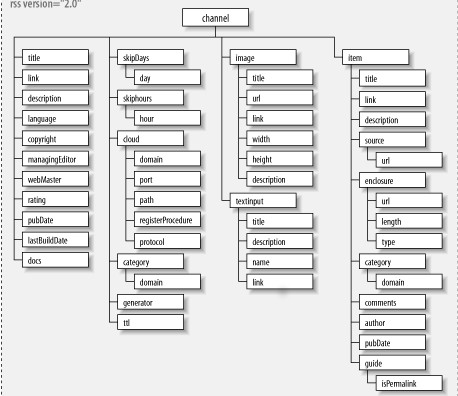
\includegraphics[scale=0.8]{rss020}
	}
	\captionof{figure}{Los elementos XML que componen RSS 2.0}
	\source{fuente: \cite{johnson2006rss}}
	\label{Los elementos XML que componen RSS 2.0}
\end{minipage}

\subsection{Plataforma Educativa LAEL}

En la Figura \ref{Subscriptor Programa Aprendizaje Francés Básico} un
usuario de sistema suscrito a un canal de noticia (francés básico); el
usuario debe iniciar sesión. 

\begin{minipage}{1.0\linewidth}
	\centering
	\fbox{
		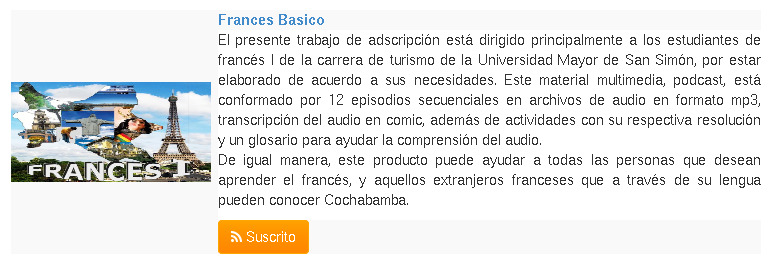
\includegraphics[scale=0.6]{basicFranceSubscribed}
	}
	\captionof{figure}{Subscriptor Programa Aprendizaje Francés Básico}
	\source{fuente: (Elaboración Propia)}
	\label{Subscriptor Programa Aprendizaje Francés Básico}
\end{minipage}

En la Figura \ref{Episodio: Elemento canal de noticias} navegador Firefox
utiliza como lector de noticias.

Estructura de un feed de noticia: Título, Fecha para Liberación y Descripción.
 
\begin{minipage}{1.0\linewidth}
	\centering
	\fbox{
		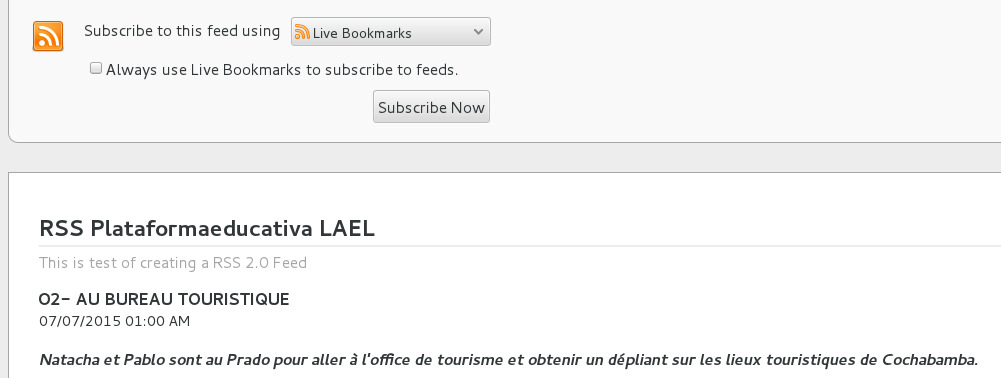
\includegraphics[scale=0.4]{basicFranceRssFirefox}
	}
	\captionof{figure}{Episodio: Elemento canal de noticias}
	\source{fuente: (Elaboración Propia)}
	\label{Episodio: Elemento canal de noticias}
\end{minipage}

\section{El nuevo estándar: Atom}

Atom es otro tipo de feed compuesto por una serie de items (elementos)
conocido como entries (entradas).

\subsection{Información básica de Atom}

Los nombres se describen a continuación:

\begin{itemize}

\item \textbf{feed} contiene el título de la fuente de noticia.
\item \textbf{author} incluye información sobre el autor.
\item \textbf{updated} indica la última fecha de actualización.
\item \textbf{id} contiene una URI que identifica de forma única el feed.
\item \textbf{link} hace referencia a una versión diferente del contenido y de la
URI de Atom.

\end{itemize}

Según \cite{wittenbrink2005rss} estos elementos son obligatorios del un
elemento feed. Si esta información no se encuentra presente un documento
Atom es considerado no válido.

\subsection{Los elementos de Atom}

En la Figura \ref{Los elementos XML que conforman un servicio de noticias Atom}
se resume la estructura de forma gráfica de un documento XML; para implementar
un feed de tipo Atom.

\begin{figure}[!ht]
	\centering
	\fbox{
		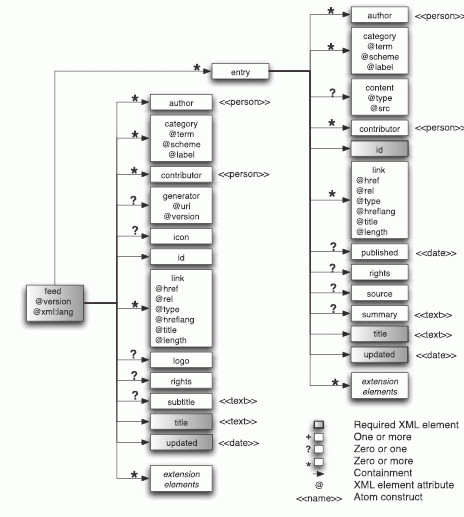
\includegraphics[scale=0.8]{elementsXML}
	}
	\caption{Los elementos XML que conforman un servicio de noticias Atom}
	\source{fuente: \cite{johnson2006rss}}
	\label{Los elementos XML que conforman un servicio de noticias Atom}
\end{figure}